\documentclass{beamer}
\usetheme{Madrid}
\beamertemplatenavigationsymbolsempty
\usepackage{graphicx}
\usepackage{pgf-soroban}
\usepackage{amsfonts}
\usepackage{amsmath}
\usepackage{xcolor}
\usepackage{tikz}
\usetikzlibrary{shapes.geometric,calc,decorations.text}
\usepackage{stmaryrd}
\usepackage{circledsteps}
\usepackage{epigraph}
\usepackage{mathtools}
\usepackage{dsfont}
\usepackage{bussproofs}
\usepackage{hyperref}
\usepackage{fontspec}
\usepackage{array}
\usepackage{bm}
\usepackage{emoji}
\setmonofont{JetBrains Mono}[
    Contextuals = Alternate,
    Ligatures = TeX,
]
\usepackage{listings}
\lstset{
    basicstyle = \ttfamily,
    columns = flexible,
}
\makeatletter
\renewcommand*\verbatim@nolig@list{}
\makeatother
\usepackage{amssymb}
\usepackage{pmboxdraw}
\usetikzlibrary{cd}
\usepackage{adjustbox}

\usepackage{tikz-3dplot}
\usetikzlibrary{3d}
\usetikzlibrary{calligraphy}
\newif\ifshowcellnumber
\showcellnumbertrue

\lstdefinelanguage{Kotlin}{
    basicstyle = \footnotesize\ttfamily,
    comment=[l]{//},
    commentstyle={\color{gray}\ttfamily},
    emph={delegate, filter, lazy, println, return@, K, E, X, P},
    emphstyle={\color{red}},
    identifierstyle=\color{black},
    keywords={abstract, actual, as, as?, break, by, class, companion, continue, data, do, dynamic, else, enum, expect, false, final, for, fun, get, if, import, in, interface, internal, is, null, object, operator, override, package, private, public, return, sealed, set, super, suspend, this, throw, true, try, typealias, tailrec, val, var, vararg, when, where, while},
    keywordstyle={\color{blue}\bfseries},
    morecomment=[s]{/*}{*/},
    morestring=[b]",
    morestring=[s]{"""*}{*"""},
    ndkeywords={@Deprecated, @JvmField, @JvmName, @JvmOverloads, @JvmStatic, @JvmSynthetic, Array, Byte, Double, Float, Int, Integer, Iterable, Long, Runnable, Short, String, Bool, Boolean},
    ndkeywordstyle={\color{orange}\bfseries},
    sensitive=true,
    stringstyle={\color{green}\ttfamily},
    showstringspaces=false,
    escapechar=@
}

\title[Probabilistic Array Programming on $\mathbb{F}_2^n$]{Probabilistic Array Programming on Galois Fields}
\author[Considine, Guo, Si]{\textbf{Breandan Considine}, Jin Guo, Xujie Si}
\institute[McGill]{
    McGill University, Mila IQIA\\
    \medskip
    \textit{breandan.considine@mail.mcgill.ca}
}
\date{\today}

\begin{document}
    \begin{frame}
        \titlepage
    \end{frame}

    \begin{frame}
        \frametitle{Overview}
        \tableofcontents
    \end{frame}

    \section{Finite Fields}\label{sec:finite-fields}


    \begin{frame}
        \frametitle{Facts about finite fields}
        \begin{itemize}
        \item Galois fields are fields which contain a finite number of elements.
        \item For every prime number p and positive integer n, there exists a finite field with $p^n$ elements, denoted $GF(p^n)$, $\mathbb{Z}/p^n$ or $\mathbb{F}_p^n$.
        \item The following instruction sets have identical expressivity:
        \begin{itemize}
        \item Pairs: $\{\vee, \neg\}, \{\wedge, \neg\}, \{\to, \neg\}, \{\to, \bot\}, \{\to, \veebar\}, \ldots$
        \item Triples: $\{\lor, =, \veebar\}, \{\lor, \veebar, \top\}, \{\land, =, \bot\}, \{\land, =, \veebar\}, \underline{\{\land, \veebar, \top\}}, \ldots$
        \end{itemize}
        \item In other words, we can compute any Boolean function $\mathbb{B}^n\rightarrow\mathbb{B}$ by composing any one of the above operator sets in an orderly fashion.
        \item $\mathbb{F}_2$ corresponds to arithmetic modulo 2, i.e., $\oplus := \veebar, \otimes := \land$.
        \item There are (at least) two schools of thought about Boolean functions:
        \begin{itemize}
        \item Logical: Conjunctive normal form. Not necessarily unique.
        \item Algebra: Algebraic normal form. It is unique.
        \end{itemize}
        \item The type $\mathbb{F}_2^n\rightarrow\mathbb{F}_2^m$ possesses $2^{m^{2^{n}}}$ inhabitants.
        \item The night before Evariste Galois was shot in a finite field, he spent writing about algebra.
        \end{itemize}
    \end{frame}

    \begin{frame}
        \frametitle{Preface to “Two Memoirs on Pure Analysis”}
        \setlength{\epigraphwidth}{0.97\textwidth}
        \epigraph{``\textit{Long algebraic calculations were at first hardly necessary for mathematical progress... It was only since Euler that concision has become indispensable to continuing the work this great geometer has given to science. Since Euler, calculation has become more and more necessary and... the algorithms so complicated that progress would be nearly impossible without the elegance that modern geometers have brought to bear on their research, and by which means the mind can promptly and with a glance grasp a large number of operations.}\\

        \vspace{5pt}
        \ldots\\
        \vspace{5pt}

        \textit{It is clear that elegance, so admirably and aptly named, has no other purpose.}\\

        \vspace{5pt}
        \ldots\\
        \vspace{5pt}

        \textit{Jump headlong into the calculations! Group the operations, classify them by their difficulties and not their appearances. This, I believe, is the mission of future geometers. This is the road on which I am embarking in this work.}''}{Evariste Galois, 1811-1832}
    \end{frame}
    
    \section{Algebraic Parsing}\label{sec:algebraic-parsing}

    %------------------------------------------------------------------------------------------------

    \begin{frame}
        \frametitle{Recap: Context Free Grammars}
        Suppose we have a context free grammar (CFG) $G = \langle V, \Sigma, P, S\rangle$ where $V$ is the set of nonterminals, $\Sigma$ is the terminals, $P: V\times (V \cup \Sigma)^+$ are the productions, $S\in V$ is the start symbol and $+$ is the Kleene plus.\newline\\
        %
        For example, consider the grammar $\underline{S \rightarrow S S \mid ( S ) \mid ()}$. This represents the language of balanced parentheses, e.g. $(), ()(), (()), ()(()), (()()), (())()\ldots$\newline\\
        %
        Every CFG has a normal form $P^*: V \times (V^2 \mid \Sigma)$, i.e., every production can be refactored into either $v_0 \rightarrow v_1 v_2$ or $v_0 \rightarrow \sigma$, where $v_{0\ldots2}: V$ and $\sigma: \Sigma$, e.g., $\{S \rightarrow S S \mid ( S ) \mid ()\}\Leftrightarrow^*\{S\rightarrow XR \mid SS \mid LR, L \rightarrow (, R \rightarrow ), X\rightarrow LS\}$

        \begin{center}
        \begin{tikzpicture}[font=\sffamily,breathe dist/.initial=4ex]
            \foreach \X [count=\Y,remember=\Y as \LastY] in
                {regular,context free}
                {\ifnum\Y=1
            \node[ellipse,draw,outer sep=0pt] (F-\Y) {\X};
            \else
            \path[decoration={text along path,
            text={|\sffamily|\X},text align=center,raise=0.3ex},decorate]
        let \p1=($(F-\LastY.north)-(F-\LastY.west)$)
            in (F-\LastY.west) arc(180:0:\x1 and \y1);
            \path let \p1=($([yshift=\pgfkeysvalueof{/tikz/breathe dist}]F-\LastY.north)
            -(F-\LastY.south)$),
            \p2=($(F-1.east)-(F-1.west)$),\p3=($(F-1.north)-(F-1.south)$)
            in ($([yshift=\pgfkeysvalueof{/tikz/breathe dist}]F-\LastY.north)!0.5!(F-\LastY.south)$)
            node[minimum height=\y1,minimum width={\y1*\x2/\y3},
            draw,ellipse,inner sep=0pt, fill=black!30!white] (F-\Y){};
            \fi
            }
            \foreach \X [count=\Y,remember=\Y as \LastY] in
                {regular,context free,context sensitive,recursively enumerable}
                {\ifnum\Y=1
            \node[ellipse,draw,outer sep=0pt] (F-\Y) {\X};
            \else
            \path[decoration={text along path,
            text={|\sffamily|\X},text align=center,raise=0.3ex},decorate]
        let \p1=($(F-\LastY.north)-(F-\LastY.west)$)
            in (F-\LastY.west) arc(180:0:\x1 and \y1);
            \path let \p1=($([yshift=\pgfkeysvalueof{/tikz/breathe dist}]F-\LastY.north)
            -(F-\LastY.south)$),
            \p2=($(F-1.east)-(F-1.west)$),\p3=($(F-1.north)-(F-1.south)$)
            in ($([yshift=\pgfkeysvalueof{/tikz/breathe dist}]F-\LastY.north)!0.5!(F-\LastY.south)$)
            node[minimum height=\y1,minimum width={\y1*\x2/\y3},
            draw,ellipse,inner sep=0pt] (F-\Y){};
            \fi}
        \end{tikzpicture}
        \end{center}
    \end{frame}


    \begin{frame}[fragile]
        \frametitle{Algebraic parsing, distilled}
        Given a CFG $\mathcal{G} \coloneqq \langle V, \Sigma, P, S\rangle$ in Chomsky Normal Form, we can construct a recognizer $R_\mathcal{G}: \Sigma^n \rightarrow \mathbb{B}$ for strings $\sigma: \Sigma^n$ as follows. Let $\mathcal P(V)$ be our domain, $0$ be $\varnothing$, $\oplus$ be $\cup$, and $\otimes$ be defined as follows:

        \vspace{-7pt}
        \[
            s_1 \otimes s_2 \coloneqq \{C \mid \langle A, B\rangle \in s_1 \times s_2, (C\rightarrow AB) \in P\}\\
            \text{E.g.},
                \{A \rightarrow BC, C \rightarrow AD, D \rightarrow BA\} \subseteq P \vdash \{A, B, C\} \otimes \{B, C, D\} = \{A, C\}
        \]
        \vspace{16pt}

        \noindent By initializing $\mathbf{M}_0[i, j](\mathcal{G}, \sigma) \coloneqq \{A \mid i + 1 = j, (A \rightarrow \sigma_i) \in P\}$ and searching for the least solution to $\mathbf{M} = \mathbf{M} + \mathbf{M}^2$, this will produce a matrix $\mathbf{M}^*$:

        \vspace{-5}
        \[
            \mathbf{M}^* = \begin{pmatrix}
                               \varnothing & \{V\}_{\sigma_1} & \ldots & \ldots & \mathcal{T} \\
                               \varnothing & \varnothing & \{V\}_{\sigma_2} & \ldots & \ldots \\
                               \varnothing & \varnothing & \varnothing & \{V\}_{\sigma_3} & \ldots \\
                               \varnothing & \varnothing & \varnothing & \varnothing & \{V\}_{\sigma_4} \\
                               \varnothing & \varnothing & \varnothing & \varnothing & \varnothing
            \end{pmatrix}
        \]

        \noindent Valiant (1975) shows that $\sigma \in \mathcal{L}(\mathcal{G})$ iff $S \in \mathcal{T}$, i.e., $\mathds{1}_{\mathcal{T}}(S) \iff \mathds{1}_{\mathcal{L}(\mathcal{G})}(\sigma)$.
    \end{frame}

    \begin{frame}[fragile]
        \frametitle{Kotlin implementation: CFG definition}
        \begin{lstlisting}[language=Kotlin, gobble=8, basicstyle=\scriptsize\ttfamily]
        typealias Production = Pair<String, List<String>>
        typealias CFG = Set<Production>
        val Production.LHS: String get() = first
        val Production.RHS: List<String> get() = second
        val CFG.nonterminals: Set<String> by cache { map { it.LHS }.toSet() }
        val CFG.words: Set<String> by cache { nonterminals + flatMap { it.RHS } }
        val CFG.terminals: Set<String> by cache { words - nonterminals }
        // Many-to-many mapping of nonterminals to RHS expansions
        val CFG.bimap: BidirectionalMap by cache { BidirectionalMap(this) }

        fun CFG.makeAlgebra(): Ring<Set<String>> =
          Ring.of(
            // 0 = @\color{gray}\texttt{∅}@
            nil = setOf(),
            // x + y = x @\color{gray}\texttt{∪}@ y
            plus = { x, y -> x union y },
            // x · y = { A0 | A1 @\color{gray}\texttt{∈}@ x, A2 @\color{gray}\texttt{∈}@ y, (A0 -> A1 A2) @\color{gray}\texttt{∈}@ P }
            times = { x, y -> join(x, y) }
          )

        fun CFG.join(ls: Set<String>, rs: Set<String>): Set<String> =
          (ls * rs).flatMap { (l, r) -> bimap[listOf(l, r)] }.toSet()
        \end{lstlisting}
    \end{frame}

    \begin{frame}[fragile]
        \frametitle{Kotlin implementation: the recognizer}
        \begin{lstlisting}[language=Kotlin, gobble=8, basicstyle=\scriptsize\ttfamily]
        // Constructs initial matrix according to: M@\color{gray}\textsubscript{i+1=j}@ = { A | (A -> @\color{gray}\texttt{σ}\textsubscript{i}@) @\color{gray}\texttt{∈}@ P }
        fun CFG.initialMatrix(str: List<String>): Matrix<Set<String>> =
          Matrix(makeAlgebra(), str.size + 1) { i, j ->
            // Aligns nonterminals matching each terminal along superdiagonal
            if (i + 1 != j) emptySet() else bimap[listOf(str[j - 1])].toSet()
          }

        // Computes the fixpoint of an abstract matrix function
        tailrec fun <T: Matrix<S>, S> T.seekFixpoint(op: (T) -> T): T {
          val next = op(this)
          return if (this == next) next else next.seekFixpoint(op)
        }

        // Checks whether start symbol is contained in the northeasternmost entry
        fun CFG.check(s: String): Boolean = START in parse(tokenize(s))[0].last()

        // Since matrix is strictly UT, this converges in at most |tokens| steps
        fun CFG.parse(tokens: List<String>): Matrix<Set<String>> =
            initialMatrix(tokens).seekFixpoint { it + it * it }
        \end{lstlisting}
    \end{frame}


    \begin{frame}
        \frametitle{A few observations on algebraic parsing}
        \begin{itemize}
            \item The matrix $\mathbf M^*$ is strictly upper triangular, i.e., nilpotent of degree $n$
            \item Recognizer can be translated into a parser by storing backpointers\\\\
        \end{itemize}\vspace{0.2cm}
        \begin{tabular}{ c c c }
            \small{$\mathbf{M}_1 = \mathbf{M}_0 + \mathbf{M}_0^2$} & \small{$\mathbf{M}_2 = \mathbf{M}_1 + \mathbf{M}_1^2$} & \small{$\mathbf{M}_3 = \mathbf{M}_2 + \mathbf{M}_2^2 = \mathbf{M}_4$} \\
            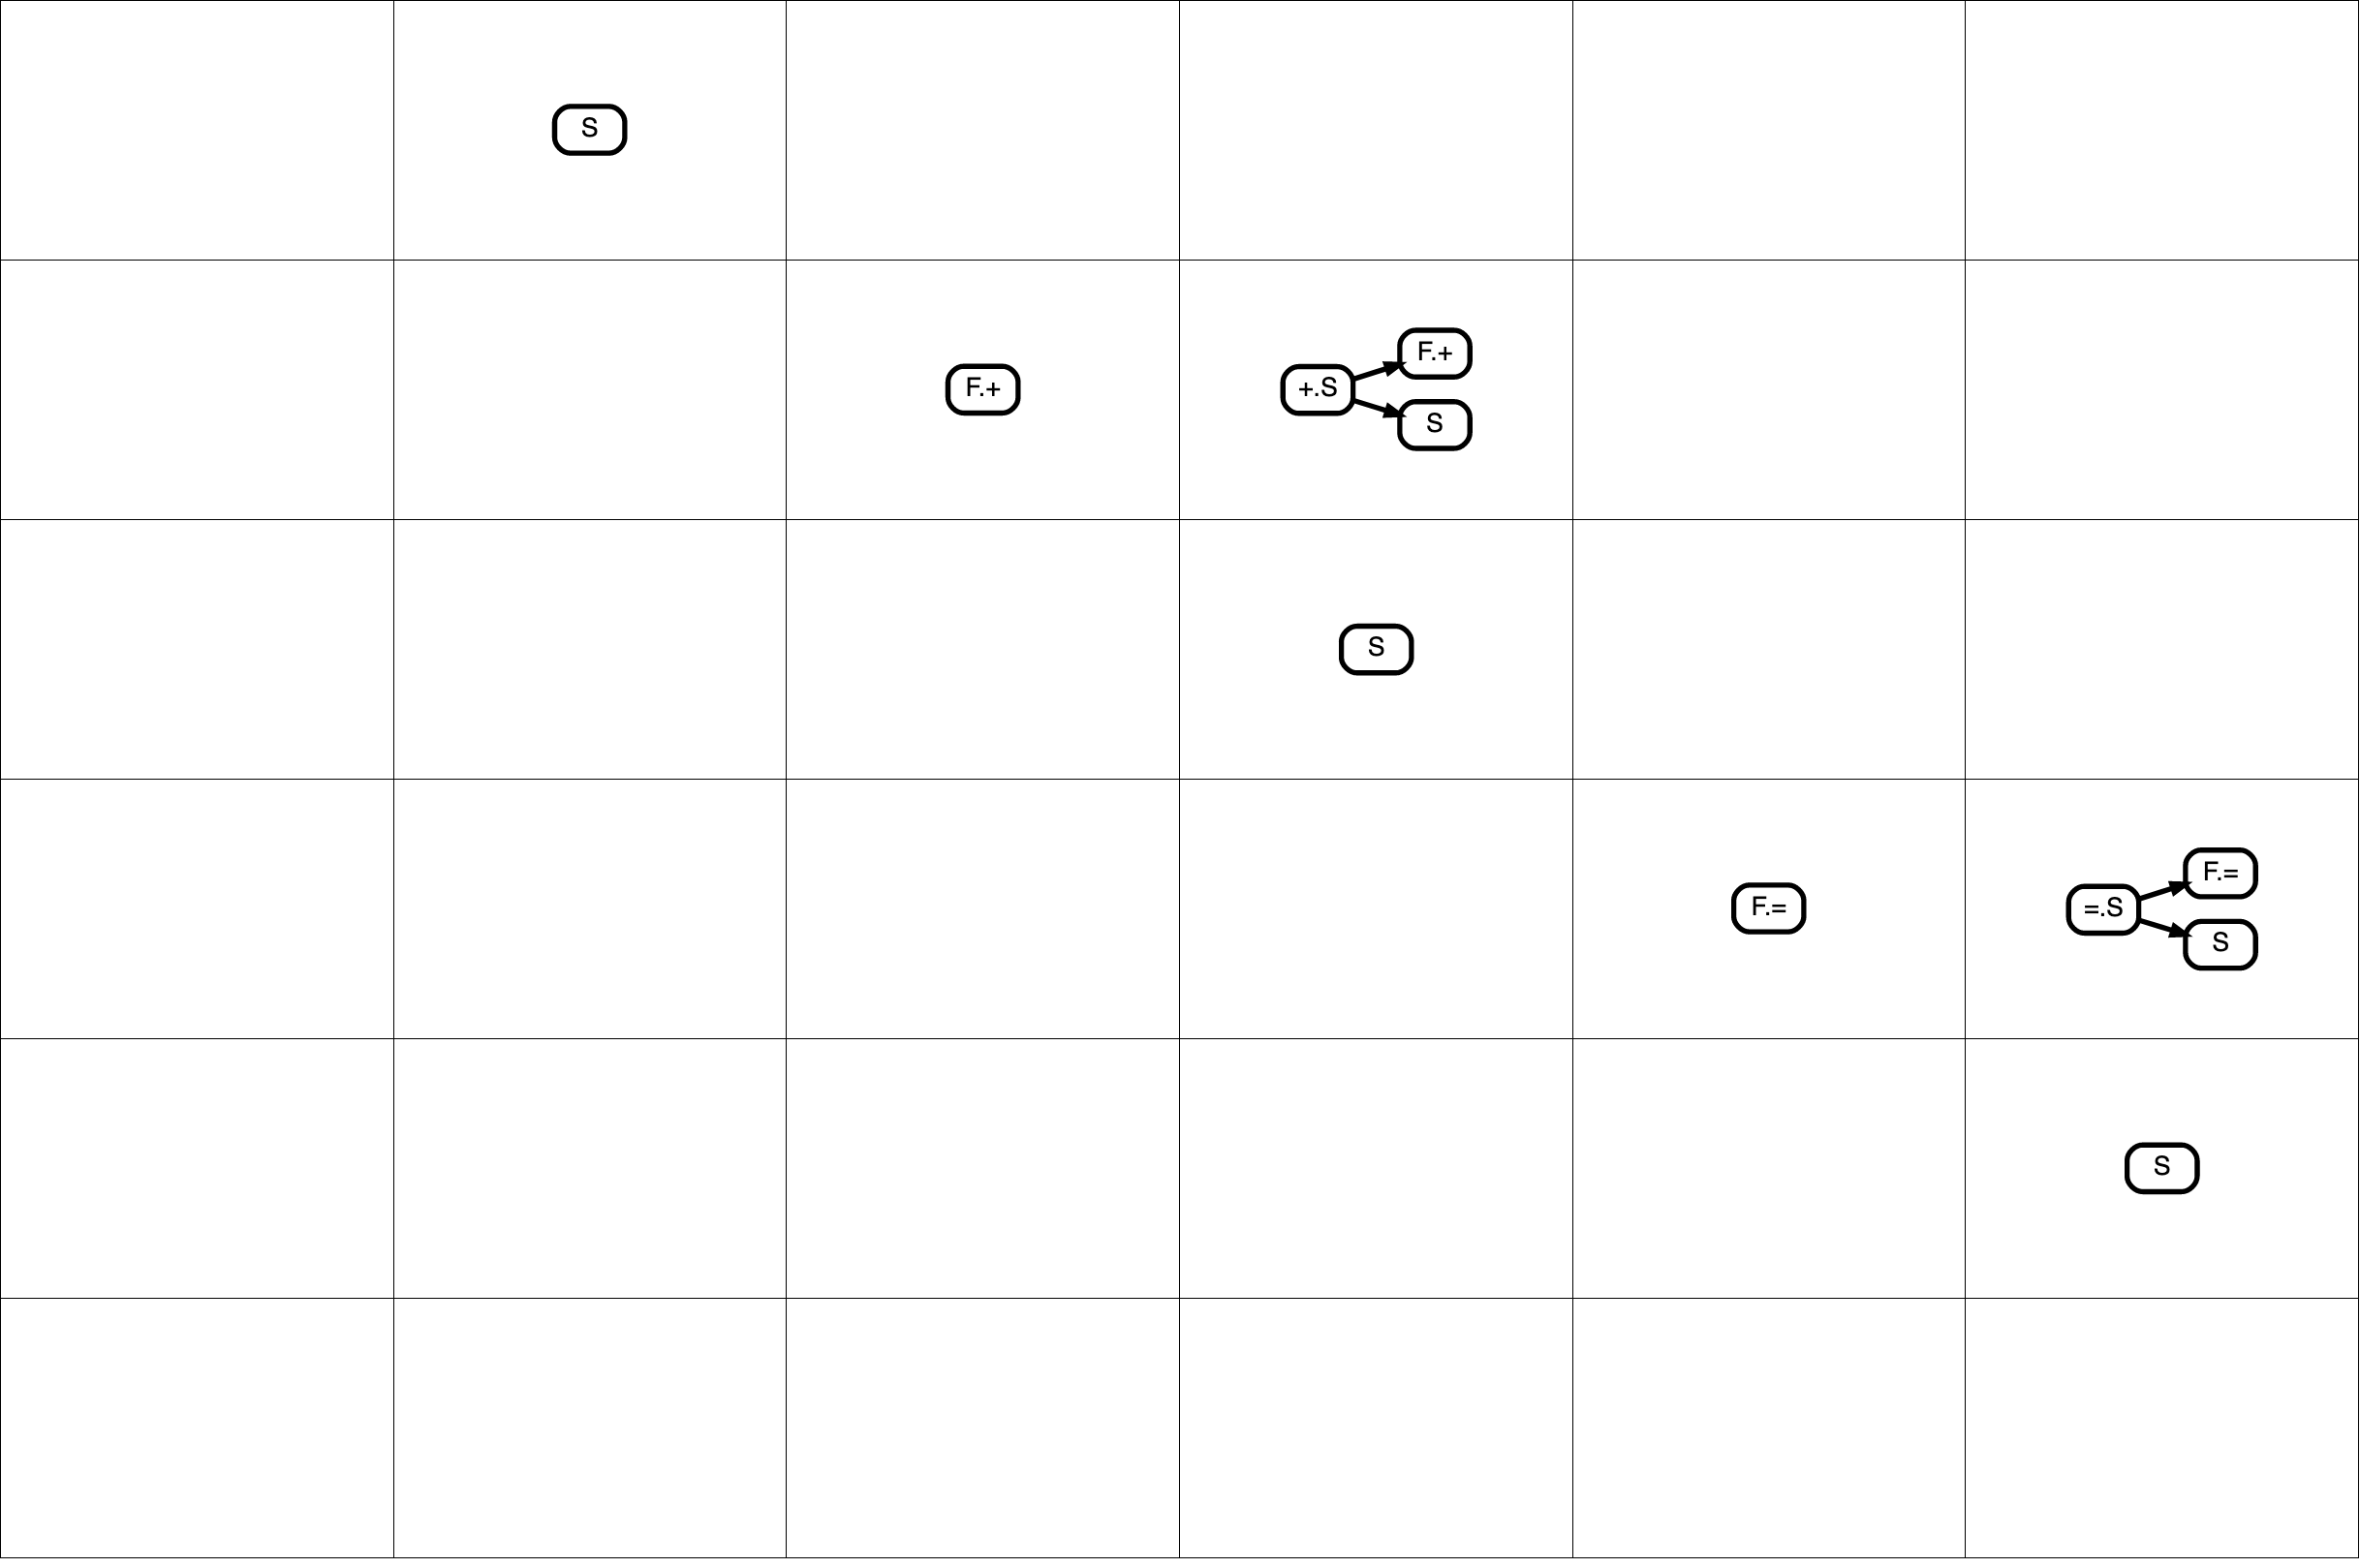
\includegraphics[trim=420 288 0 0,clip, width=3.6cm]{../figures/parse2.png} &
            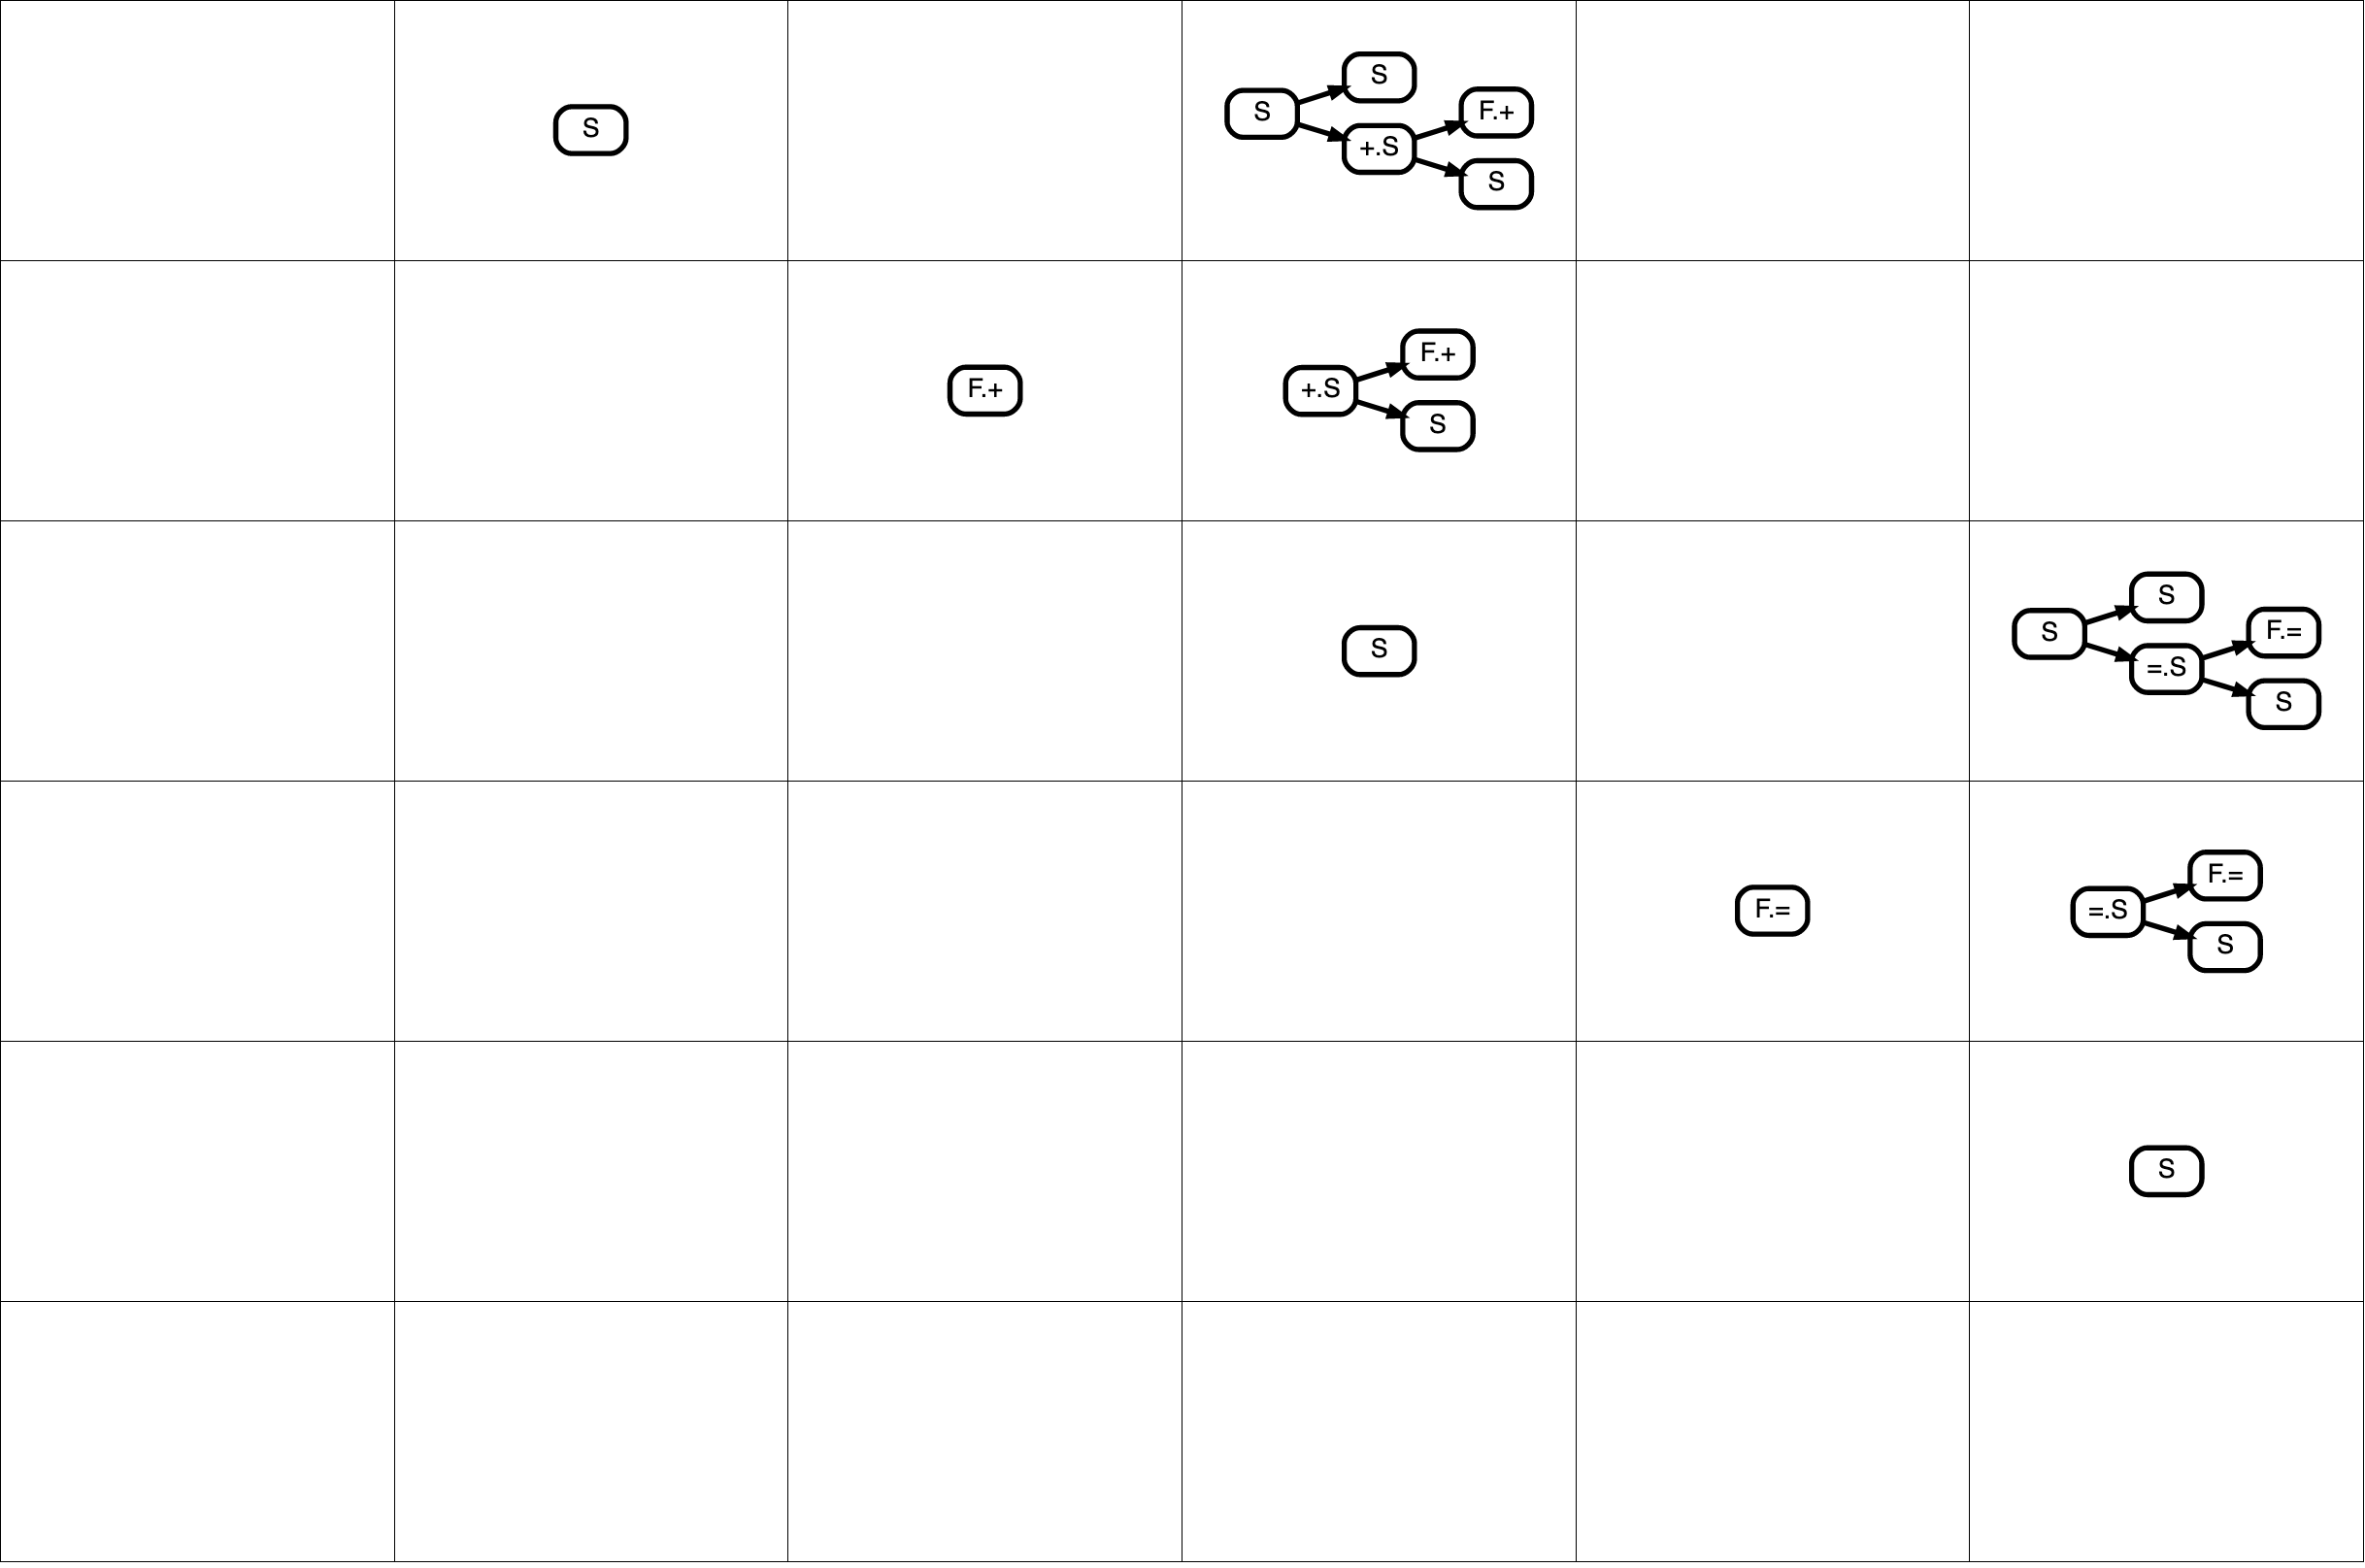
\includegraphics[trim=420 285 0 0,clip, width=3.6cm]{../figures/parse3.png} &
            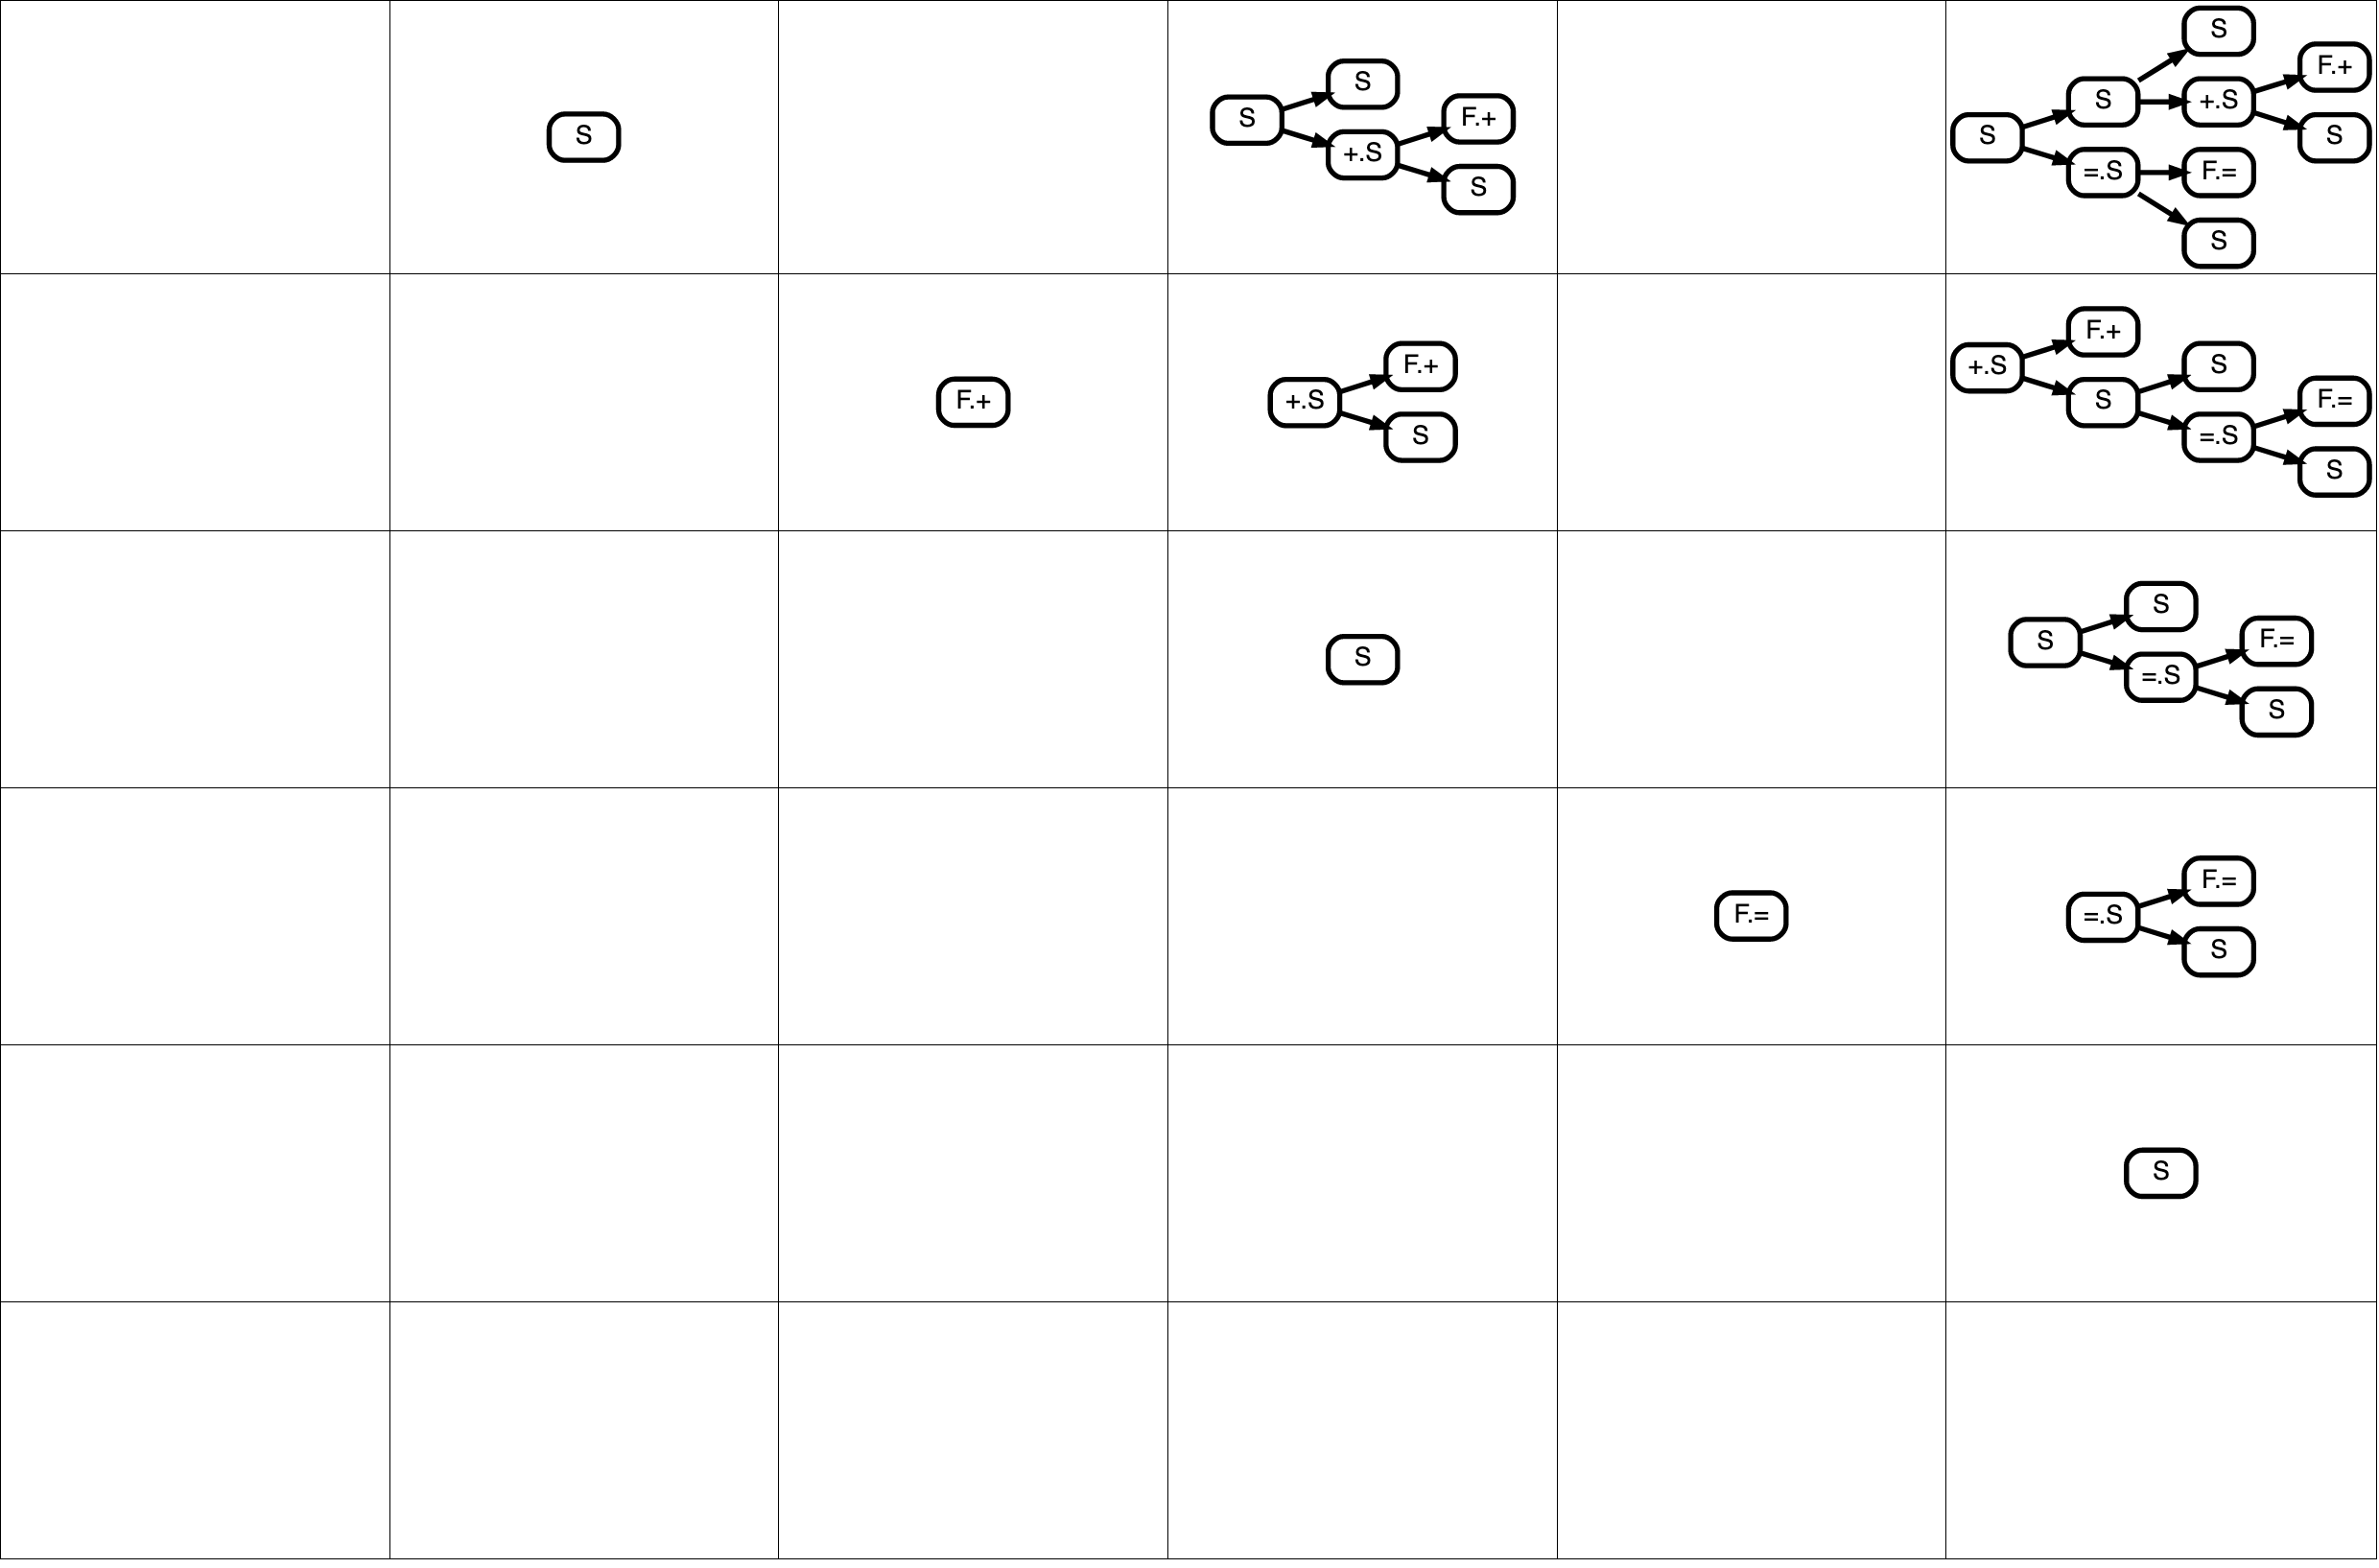
\includegraphics[trim=420 287 0 0,clip, width=3.63cm]{../figures/parse4.png}
        \end{tabular}
        \begin{itemize}
            \item The $\otimes$ operator is \textit{not} associative: $S \otimes (S \otimes S) \neq (S \otimes S) \otimes S$
            \item Built-in error recovery: nonempty submatrices = parsable fragments
            \item \texttt{seekFixpoint \{ it + it * it \}} is sufficient but unnecessary
            \item If we had a way to solve for $\mathbf{M = M + M}^2$ directly, power iteration would be unnecessary, could solve for $\mathbf{M = M}^2$ above superdiagonal
        \end{itemize}
    \end{frame}

    \begin{frame}[fragile]
        \frametitle{Satisfiability + holes (our contribution)}
        \begin{itemize}
            \item Can be lowered onto a Boolean tensor $\mathbb{B}^{n\times n \times |V|}$ (Valiant, 1975)
            \item Binarized CYK parser can be efficiently compiled to a SAT solver
            \item Enables sketch-based synthesis in either $\sigma$ or $\mathcal G$: just use variables!
            \item We simply encode the characteristic function, i.e. $\mathds{1}_{\subseteq V}: V\rightarrow \mathbb{B}^{|V|}$
            \item $\oplus, \otimes$ are defined as $\boxplus, \boxtimes$, so that the following diagram commutes:
            \[\begin{tikzcd}
                  V \times V \arrow[r, "\oplus/\otimes"] \arrow[d, "\mathds{1}^2"]
                  & V \arrow[d, "\mathds{1}\phantom{^{-1}}"] \\
                  \mathbb{B}^{|V|} \times \mathbb{B}^{|V|} \arrow[r, "\boxplus/\boxtimes", labels=below] \arrow[u, "\mathds{1}^{-2}"]
                  & \mathbb{B}^{|V|} \arrow[u, "\mathds{1}^{-1}"]
            \end{tikzcd}\]
            \item These operators can be lifted into matrices/tensors in the usual way
            \item In most cases, only a few nonterminals are active at any given time
            \item More sophisticated representations are known for $\binom{n}{0 \leq k}$ subsets
            \item If density is desired, possible to use the Maculay representation
%            \item Set joins are an active topic of research in SQL query optimization
            \item If you know of a more efficient encoding, please let us know!
        \end{itemize}
    \end{frame}

    \begin{frame}[fragile]
        \frametitle{Tidyparse IDE plugin}
        \href{https://github.com/breandan/tidyparse}{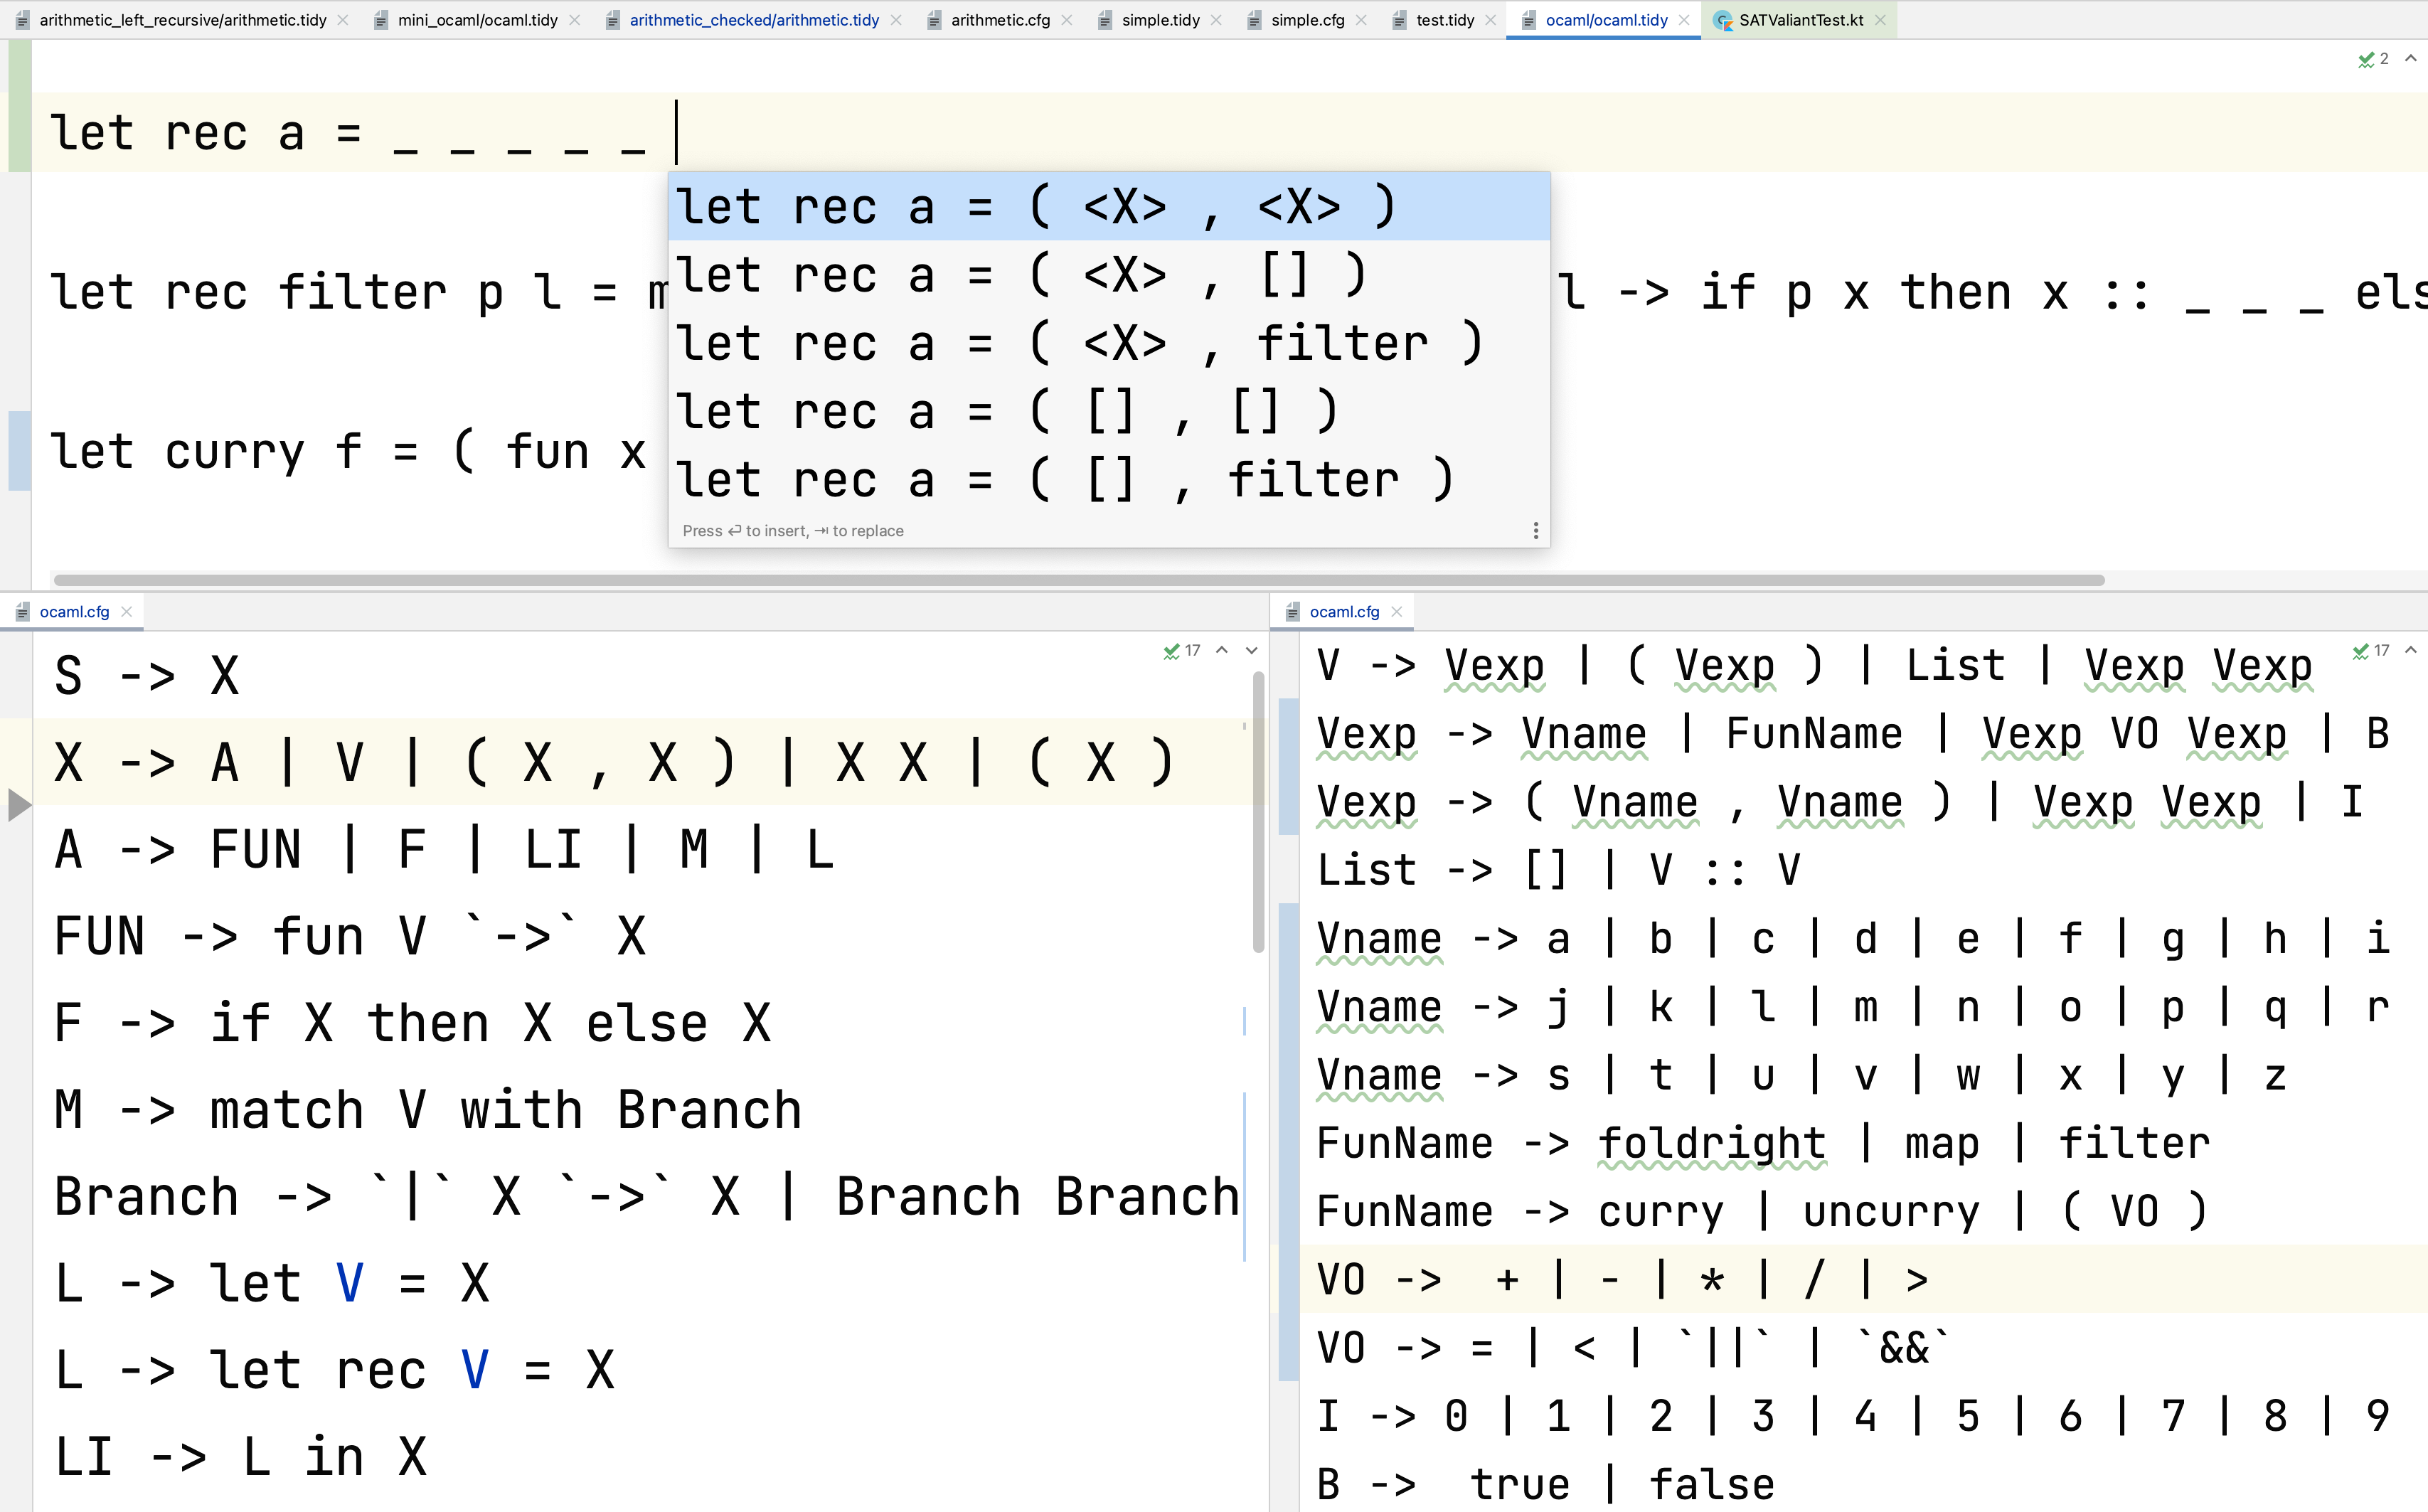
\includegraphics[width=\textwidth]{../figures/tidyparse.png}}
    \end{frame}

    \begin{frame}
        \frametitle{Abbreviated history of algebraic parsing}
        \begin{itemize}
            \item \href{http://www-igm.univ-mlv.fr/~berstel/Mps/Travaux/A/1963-7ChomskyAlgebraic.pdf}{Chomsky \& Sch\"utzenberger (1959) - The algebraic theory of CFLs}
            \item Cocke–Younger–Kasami (1961) - Bottom-up matrix-based parsing
            \item \href{https://dl.acm.org/doi/10.1145/321239.321249}{Brzozowski (1964) - Derivatives of regular expressions}
            \item \href{https://dl.acm.org/doi/10.1145/362007.362035}{Earley (1968) - top-down dynamic programming (no CNF needed)}
            \item \href{http://theory.stanford.edu/~virgi/cs367/papers/valiantcfg.pdf}{Valiant (1975) - first realizes the Boolean matrix correspondence}
            \begin{itemize}
                \item Na\"ively, has complexity $\mathcal{O}(n^4)$, can be reduced to $\mathcal{O}(n^\omega)$, $\omega < 2.763$
            \end{itemize}
            \item \href{https://www.cs.cornell.edu/home/llee/papers/bmmcfl-jacm.pdf}{Lee (1997) - Fast CFG Parsing $\Longleftrightarrow$ Fast BMM, formalizes reduction}
            \item \href{https://matt.might.net/papers/might2011derivatives.pdf}{Might et al. (2011) - Parsing with derivatives (Brzozowski $\Rightarrow$ CFL)}
            \item \href{https://users.math-cs.spbu.ru/~okhotin/papers/formal_languages_gf2.pdf}{Bakinova, Okhotin et al. (2010) - Formal languages over GF(2)}
            \item \href{https://arxiv.org/pdf/1601.07724.pdf}{Bernady \& Jansson (2015) - Certifies Valiant (1975) in Agda}
            \item \href{https://arxiv.org/pdf/1504.08342.pdf}{Cohen \& Gildea (2016) - Generalizes Valiant (1975) to parse and recognize mildly context sensitive languages, e.g. LCFRS, TAG, CCG}
            \item \textbf{Considine, Guo \& Si (2022) - SAT + Valiant (1975) + holes}
        \end{itemize}
    \end{frame}

    \section{Typelevel Arithmetic}

    \begin{frame}
        \frametitle{Abacus arithmetic}
        \begin{itemize}
        \item Computational complexity of arithmetic is notation-dependent(!)
        \item For example, $\pm$ in unary arithmetic is concatenation and decatenation
        \item Multiplication and division by natural powers of the radix is $\mathcal{O}(1)$
        \item We can describe the abacus as a kind of abstract rewriting system
        \end{itemize}
        \ladj{0.25}
        \begin{prooftree}
            \AxiomC{
                \tikz \fill [white] (0,0) rectangle (1,2);
            }
            \UnaryInfC{
                \begin{tikzpicture}
                    \tige{1}{0}{0}
                    \tige{2}{0}{0}
                    \tige{3}{0}{0}
                    \cadre{3}
                \end{tikzpicture}
            }
            \DisplayProof
            \hskip 1em
            \AxiomC{
                \begin{tikzpicture}
                    \tige{1}{0}{0}
                    \barres{1}
                \end{tikzpicture}$_n+10^n$
            }
            \UnaryInfC{
                \begin{tikzpicture}
                    \tige{1}{1}{0}
                    \barres{1}
                \end{tikzpicture}$_n\phantom{n+0^n}$
            }
            \DisplayProof
            \hskip 1em
            \AxiomC{
                \begin{tikzpicture}
                    \tige{1}{4}{0}
                    \barres{1}
                \end{tikzpicture}$_n+10^n$
            }
            \UnaryInfC{
                \begin{tikzpicture}
                    \tige{1}{5}{0}
                    \barres{1}
                \end{tikzpicture}$_n\phantom{n+0^n}$
            }
            \DisplayProof
            \hskip 1em
            \AxiomC{
                \begin{tikzpicture}
                    \tige{1}{0}{0}
                    \barres{1}
                    \tige[2]{1}{9}{0}
                    \barres[2]{1}
                \end{tikzpicture}$_n+10^n$
            }
            \UnaryInfC{
                \begin{tikzpicture}
                \tige{1}{1}{0}
                \barres{1}
                \tige[2]{1}{0}{0}
                \barres[2]{1}
                \end{tikzpicture}$_n\phantom{n+0^n}$
            }
        \end{prooftree}
    \end{frame}

    \begin{frame}[fragile]
        \frametitle{Abacus dependent types}
        \begin{lstlisting}[language=Kotlin, gobble=7]
        sealed class B<X, P : B<X, P>>(open val x: X? = null) {
          val T: T<P> get() = T(this as P)
          val F: F<P> get() = F(this as P)
        }

        class U(val i: Int) : B<Any, U>() // Checked at runtime

        object Ø: B<Ø, Ø>(null) // Denotes the end of a bitlist

        class T<X>(override val x: X = Ø as X) : B<X, T<X>>(x)
          { companion object: T<Ø>(Ø) }

        class F<X>(override val x: X = Ø as X) : B<X, F<X>>(x)
          { companion object: F<Ø>(Ø) }

        val b0: F<Ø> = F
        val b1: T<Ø> = T
        val b2: F<T<Ø>> = T.F // Note the raw type is reversed
        val b4: F<F<T<Ø>>> = T.F.F
        \end{lstlisting}
    \end{frame}

    \begin{frame}[fragile]
        \frametitle{Abacus dependent types}
        \begin{lstlisting}[language=Kotlin, gobble=7]
        typealias B_0<K> = F<K> // Type synonyms for legibility
        typealias B_1<K> = T<K>
        typealias B_2<K> = F<T<K>>
        typealias B_3<K> = T<T<K>>
        typealias B_4<K> = F<F<T<K>>>
        typealias B_7<K> = T<T<T<K>>>
        typealias B_8<K> = F<F<F<T<K>>>>

        // Calculates k + 1 for all k == 2@\color{gray}\textsuperscript{n}@ - 1, 0 <= n < 4
        operator fun Ø.plus(t: T<Ø>) = b1
        operator fun B_0<Ø>.plus(t: T<Ø>) = b1
        operator fun B_1<Ø>.plus(t: T<Ø>): B_2<Ø> = F(x + b1)
        operator fun B_3<Ø>.plus(t: T<Ø>): B_4<Ø> = F(x + b1)
        operator fun B_7<Ø>.plus(t: T<Ø>): B_8<Ø> = F(x + b1)

        // Calculates k + 1 for all k @≡@ 2@\color{gray}\textsuperscript{n}@ - 1 (mod 2@\color{gray}\textsuperscript{n+1}@), 1 <= n < 4
        operator fun <K: B<*, *>> B_0<K>.plus(t: T<Ø>) = T(x)
        operator fun <K: B<*, *>> B_1<F<K>>.plus(t: T<Ø>) = F(x + b1)
        operator fun <K: B<*, *>> B_3<F<K>>.plus(t: T<Ø>) = F(x + b1)
        operator fun <K: B<*, *>> B_7<F<K>>.plus(t: T<Ø>) = F(x + b1)
        \end{lstlisting}
    \end{frame}

    \begin{frame}[fragile]
        \frametitle{Abacus dependent types: birds eye view}
        \begin{tiny}
        \begin{verbatim}
             i\j│  0  1  …  k-1  k  │  k+1  k+2  …  k+c  │  k+c+1  …  k+c+d-1
             ───┼───────────────────┼────────────────────┼────────────────────┐
              0 │                   │                    │                  __|
              1 │                   │                    │               __/░░
              … │       i ± j       │        i + j       │            __/░░░░░
              … │       j ± i       │        j ± i       │         __/░░░░░░░░
            k-1 │                   │                    │      __/░░░░░░░░░░░
              k │                   │                    │   __╱░░░░░░░░░░░░░░
            ────┼───────────────────┼────────────────────┴──┘░░░░░░░░░░░░░░░░░
            k+1 │                   │░░░░░░░░░░░░░░░░░░░░░░░░░░░░░░░░░░░░░░░░░
            k+2 │                   │░░░░░░░░░░░░░░░░░░░░░░░░░░░░░░░░░░░░░░░░░
              … │       i ± j       │░░░░░░░░░░░░░░░░░░░░░░░░░░░░░░░░░░░░░░░░░
              … │       j + i       │░░░░░░░░░░░░░░░░░░░░░░░░░░░░░░░░░░░░░░░░░
          k+c-1 │                   │░░░░░░░░░░░░                ░░░░░░░░░░░░░
            k+c │                   │░░░░░░░░░░░░    Run-time    ░░░░░░░░░░░░░
           ─────┼───────────────────┤░░░░░░░░░░░░                ░░░░░░░░░░░░░
          k+c+1 │                __/░░░░░░░░░░░░░  type checked  ░░░░░░░░░░░░░
          k+c+2 │             __/░░░░░░░░░░░░░░░░                ░░░░░░░░░░░░░
              … │          __/░░░░░░░░░░░░░░░░░░░░░░░░░░░░░░░░░░░░░░░░░░░░░░░░
              … │       __/░░░░░░░░░░░░░░░░░░░░░░░░░░░░░░░░░░░░░░░░░░░░░░░░░░░
        k+c+d-2 │    __/░░░░░░░░░░░░░░░░░░░░░░░░░░░░░░░░░░░░░░░░░░░░░░░░░░░░░░
        k+c+d-1 │___/░░░░░░░░░░░░░░░░░░░░░░░░░░░░░░░░░░░░░░░░░░░░░░░░░░░░░░░░░
        \end{verbatim}
        \end{tiny}
    \end{frame}

    \begin{frame}
        \frametitle{Annotated history of typed eDSLs}
        \begin{itemize}
            \item \href{https://www.cs.utexas.edu/~wcook/papers/FBound89/CookFBound89.pdf}{Canning et al. (1989) - F-Bounded Polymorphism is first invented}
            \item \href{https://ecommons.cornell.edu/bitstream/handle/1813/5614/TR2003-1901.pdf}{Cheney \& Hinze (2003) - Phantom types (good for type-safe builders)}
            \item \href{https://dl.acm.org/doi/pdf/10.1145/1142473.1142552}{Meijer et al. (2006) - Language integrated querying (LINQ)}
            \item \href{https://jooq.org}{Eder (2011) - Commercial reimplementation LINQ in Java/jOOQ}
            \item \href{https://arxiv.org/pdf/1605.05274.pdf}{Grigore (2016) - Java Generics shown to be Turing Complete}
            \item \href{https://github.com/erdos/java-logic}{Erdős (2017) - Encodes Boolean logic into Java type system}
            \item \href{https://dl.acm.org/doi/10.1145/3136040.3136041}{Nakamaru et al. (2017) - Silverchain: a fluent API generator}
            \item \href{http://breandan.net/public/masters_thesis.pdf#2}{\textbf{Considine (2019) - Shape-safe matrix multiplication in Kotlin$\nabla$}}
            \item \href{https://drops.dagstuhl.de/opus/volltexte/2019/10805/pdf/LIPIcs-ECOOP-2019-13.pdf}{Gil \& Roth (2019) - Fling, a fluent API parser generator}
            \item \href{https://arxiv.org/pdf/2109.03950.pdf}{Roth (2021) - Encodes CFL into Nominal Subtyping with Variance}
            \item \href{https://github.com/breandan/galoisenne}{\textbf{Considine (2021) - Arithmetic in Kotlin via typelevel abacus}}
            \item We know how to lower parsing onto types, what about vis versa?
        \end{itemize}
    \end{frame}

    \begin{frame}[fragile]
        \frametitle{Can we lower type checking onto parsing?}
        First, let us consider the untyped version:
        \begin{lstlisting}[language=Kotlin, gobble=5]
        Exp -> 0 | 1 | ... | T | F
        Exp -> Exp Op Exp | if ( Exp ) Exp else Exp
        Op -> and | or | + | *
        \end{lstlisting}
        Now, let us consider the GADT/HOAS version:
        \begin{lstlisting}[language=Kotlin, gobble=5]
        Exp<Bool> -> T | F
        Op<Bool> -> and | or
        Exp<Int> -> 0 | 1 | ... | 9
        Op<Int> -> + | *
        Exp<E> -> Exp<E> Op<E> Exp<E> // Es must be exactly the same!
        Exp<E> -> if ( Exp<Bool> ) Exp<E> else Exp<E>
        \end{lstlisting}
        We can eliminate contextuality by concretizing over \lstinline[language=Kotlin]{E -> Bool | Int}:
        \begin{lstlisting}[language=Kotlin, gobble=5]
        Exp<Bool> -> T | F
        Exp<Bool> -> Exp<Bool> or Exp<Bool> | Exp<Bool> and Exp<Bool>
        Exp<Bool> -> if ( Exp<Bool> ) Exp<Bool> else Exp<Bool>
        Exp<Int> -> 0 | 1 | ... | 9
        Exp<Int> -> Exp<Int> + Exp<Int> | Exp<Int> * Exp<Int>
        Exp<Int> -> if ( Exp<Bool> ) Exp<Int> else Exp<Int>
        \end{lstlisting}
    \end{frame}

    \section{Random Numbers}

    \begin{frame}
        \frametitle{Linear Finite State Registers}
        Let $\textbf{M}: \text{GF}(2^{n\times n})$ be a square matrix $\mathbf{M}^0_{r, c} = P_c \text{ if } r=0 \text{ else } \mathds{1}[c = r - 1]$, where $P$ is a feedback polynomial over $GF(2^n)$ with coefficients $P_{1\ldots n}$ and semiring operators $\oplus := \veebar, \otimes := \land$:\\

        \[
            \mathbf{M}^tV = \begin{pmatrix}
                                P_1 & P_2 & P_3 & P_4 & P_5 \\
                                \top & \circ & \circ & \circ & \circ \\
                                \circ & \top & \circ & \circ & \circ \\
                                \circ & \circ & \top & \circ & \circ \\
                                \circ & \circ & \circ & \top & \circ
            \end{pmatrix}^t
            \begin{pmatrix}
                V_1 \\
                V_2 \\
                V_3 \\
                V_4 \\
                V_5
            \end{pmatrix}
        \]\\

        Selecting any $V \neq \mathbf{0}$ and coefficients $P_j$ from a known \textit{primitive polynomial} then powering the matrix $\mathbf{M}$ generates an ergodic sequence over GF$(2^n)$:\\

        \[
        \mathbf{S} = \begin{pmatrix}V & \mathbf{M}V & \mathbf{M}^{2}V & \mathbf{M}^{3}V & \cdots & \mathbf{M}^{2^n-1}V \end{pmatrix}
        \]

        This sequence has \textit{full periodicity}, i.e., for all $i, j \in [0, 2^n), \mathbf{S}_i = \mathbf{S}_j \Rightarrow i = j$.
    \end{frame}

    \begin{frame}[fragile]
        \frametitle{Linear finite state registers}
        \begin{verbatim}
          1  +  x³ +  x⁵        a  b  c  d  e     V₁
 P = 20 = 0  0  1  0  1         1  0  0  0  0     V₂
          ∥  ∥  ∥  ∥  ∥         0  1  0  0  0  *  V₃
          a  b  c  d  e         0  0  1  0  0     V₄
    ╭────────── ⊗ ────╮         0  0  0  1  0     V₅
    │           │     │
    0 ──► 1  0  1  1  1 ──►           M        *  V
                ╰──┬──╯
                "taps"          S₄ = M … S₁ = M * V
                                ∥        ∥        ∥
    S₀ = 1  0  1  1  1          0        0        1
    S₁ = 0  1  0  1  1          0        1        0
    S₂ = 1  0  1  0  1          1        0        1
    S₃ = 0  1  0  1  0          0        1        1
    S₄ = 0  0  1  0  1          1        0        1
        \end{verbatim}
    \end{frame}

    \begin{frame}[fragile]
        \frametitle{Multidimensional sampling: the hasty pudding trick}
        \definecolor{R}{RGB}{202,65,55}
        \definecolor{G}{RGB}{151,216,56}
        \definecolor{B}{RGB}{0,0,0}
        \definecolor{W}{RGB}{255,255,255}
        \definecolor{X}{RGB}{65,65,65}

        \newcommand{\TikZRubikFaceLeft}[9]{\def\myarrayL{#1,#2,#3,#4,#5,#6,#7,#8,#9}}
        \newcommand{\TikZRubikFaceRight}[9]{\def\myarrayR{#1,#2,#3,#4,#5,#6,#7,#8,#9}}
        \newcommand{\TikZRubikFaceTop}[9]{\def\myarrayT{#1,#2,#3,#4,#5,#6,#7,#8,#9}}
        \newcommand{\BuildArray}{\foreach \X [count=\Y] in \myarrayL%
        {\ifnum\Y=1%
        \xdef\myarray{"\X"}%
        \else%
        \xdef\myarray{\myarray,"\X"}%
        \fi}%
        \foreach \X in \myarrayR%
        {\xdef\myarray{\myarray,"\X"}}%
        \foreach \X in \myarrayT%
        {\xdef\myarray{\myarray,"\X"}}%
        \xdef\myarray{{\myarray}}%
        }
        \TikZRubikFaceLeft
        {X}{W}{W}
        {W}{X}{X}
        {X}{W}{W}
        \TikZRubikFaceRight
        {W}{X}{W}
        {X}{W}{X}
        {W}{X}{W}
        \TikZRubikFaceTop
        {X}{W}{X}
        {W}{W}{X}
        {W}{X}{W}
        \BuildArray
        \pgfmathsetmacro\radius{0.1}
        \tdplotsetmaincoords{55}{135}

        \showcellnumberfalse


        \bgroup

        \begin{figure}
        \hspace{-0.5cm}\begin{minipage}[l]{5cm}
        \begin{tikzpicture}
        \clip (-3,-2.5) rectangle (3,2.5);
        \begin{scope}[tdplot_main_coords]
            \filldraw [canvas is yz plane at x=1.5] (-1.5,-1.5) rectangle (1.5,1.5);
            \filldraw [canvas is xz plane at y=1.5] (-1.5,-1.5) rectangle (1.5,1.5);
            \filldraw [canvas is yx plane at z=1.5] (-1.5,-1.5) rectangle (1.5,1.5);
            \foreach \X [count=\XX starting from 0] in {-1.5,-0.5,0.5}{
            \foreach \Y [count=\YY starting from 0] in {-1.5,-0.5,0.5}{
            \pgfmathtruncatemacro{\Z}{\XX+3*(2-\YY)}
            \pgfmathsetmacro{\mycolor}{\myarray[\Z]}
            \draw [thick,canvas is yz plane at x=1.5,shift={(\X,\Y)},fill=\mycolor] (0.5,0) -- ({1-\radius},0) arc (-90:0:\radius) -- (1,{1-\radius}) arc (0:90:\radius) -- (\radius,1) arc (90:180:\radius) -- (0,\radius) arc (180:270:\radius) -- cycle;
            \ifshowcellnumber
            \node[canvas is yz plane at x=1.5,shift={(\X+0.5,\Y+0.5)}] {\Z};
            \fi
            \pgfmathtruncatemacro{\Z}{2-\XX+3*(2-\YY)+9}
            \pgfmathsetmacro{\mycolor}{\myarray[\Z]}
            \draw [thick,canvas is xz plane at y=1.5,shift={(\X,\Y)},fill=\mycolor] (0.5,0) -- ({1-\radius},0) arc (-90:0:\radius) -- (1,{1-\radius}) arc (0:90:\radius) -- (\radius,1) arc (90:180:\radius) -- (0,\radius) arc (180:270:\radius) -- cycle;
            \ifshowcellnumber
            \node[canvas is xz plane at y=1.5,shift={(\X+0.5,\Y+0.5)},xscale=-1] {\Z};
            \fi
            \pgfmathtruncatemacro{\Z}{2-\YY+3*\XX+18}
            \pgfmathsetmacro{\mycolor}{\myarray[\Z]}
            \draw [thick,canvas is yx plane at z=1.5,shift={(\X,\Y)},fill=\mycolor] (0.5,0) -- ({1-\radius},0) arc (-90:0:\radius) -- (1,{1-\radius}) arc (0:90:\radius) -- (\radius,1) arc (90:180:\radius) -- (0,\radius) arc (180:270:\radius) -- cycle;
            \ifshowcellnumber
            \node[canvas is yx plane at z=1.5,shift={(\X+0.5,\Y+0.5)},xscale=-1,rotate=-90] {\Z};
            \fi
            }
            }

            \draw [decorate,decoration={calligraphic brace,amplitude=10pt,mirror},yshift=0pt, line width=1.25pt]
            (3,0) -- (3,3) node [black,midway,xshift=-8pt, yshift=-14pt] {\footnotesize $|\Sigma|$};
            \draw [decorate,decoration={calligraphic brace,amplitude=10pt},yshift=0pt, line width=1.25pt]
            (3,0) -- (0,-3) node [black,midway,xshift=-16pt, yshift=0pt] {\footnotesize $|\Sigma|$};
            \draw [decorate,decoration={calligraphic brace,amplitude=10pt},yshift=0pt, line width=1.25pt]
            (0,-3) -- (-3,-3) node [black,midway,xshift=-8pt, yshift=14pt] {\footnotesize $|\Sigma|$};
        \end{scope}
        \end{tikzpicture}
        \end{minipage}\hspace{1cm}
        \begin{minipage}[c]{5.5cm}
        To uniformly sample $\bm\sigma \sim \Sigma^n$ without replacement, we could track historical samples, or, we can form an injection $GF(2^n)\rightharpoonup\Sigma^d$, cycle a primitive polynomial over $GF(2^n)$, then discard samples that do not identify an element in any indexed dimension. This procedure rejects $(1 - |\Sigma|2^{-\lceil\log_2|\Sigma|\rceil})^d$ samples on average and requires $\sim\mathcal{O}(1)$.
        \end{minipage}
        \end{figure}
        \begin{small}
            \begin{verbatim}
                   e.g., Σ² = {A, B, C}², x⁴ + x³ + 1

   S₀     S₁     S₂     S₃     S₄     S₅     S₆     S₇
   ||     ||     ||     ||     ||     ||     ||     ||
 [1000] [0100] [0010] [1001] [1100] [0110] [1011] [0101]
  C A    B A    A C    C B           B C           B B
            \end{verbatim}
        \end{small}
    \egroup
    \end{frame}

    \begin{frame}[fragile]
        \frametitle{Multidimensional No-Replacement Sampler}

        \begin{lstlisting}[language=Kotlin, gobble=8]
        fun List<Int>.bitLens() = map { ceil(log2(it.toDouble())).toInt() }

        // Splits a bitvector into designated chunks and returns indices
        // (10101011, [3, 2, 3]) -> [101, 01, 011] -> [4, 1, 3]
        fun List<Boolean>.toIndexes(bitLens: List<Int>): List<Int> =
          bitLens.fold(listOf<List<Boolean>>() to this) { (a, b), i ->
            (a + listOf(b.take(i))) to b.drop(i)
          }.first.map { it.toInt() }

        fun Sequence<List<Boolean>>.hastyPudding(lengths: List<Int>) =
          map { it.toIndexes(lengths.bitLens()) }
           .filter { it.zip(lengths).all { (a, b) -> a < b } }

        fun <T> List<Set<T>>.sampleWithoutReplacement(
          lengths: List<Int> = map { it.size },
          bitLens: List<Int> = map(Set<T>::size).bitLens(),
          degree: Int = bitLens.sum().also { println("LFSR(GF(2^$it))") }
        ): Sequence<List<T>> =
          LFSR(degree).hastyPudding(lengths)
            .map { zip(it).map { (dims, idx) -> dims[idx] } }
        \end{lstlisting}
    \end{frame}

    \section{Future Work}

    \begin{frame}
        \frametitle{What's the point?}
        \begin{itemize}
            \item Algebraists have developed a powerful language for rootfinding
            \item Tradition handed down from Euler, Galois, Borel, Kleene, Chomsky
            \item We know closed forms for exponentials of structured matrices
%            \item Characteristic polynomials, companion matrices, eigenvalues
            \item Solving these forms can be much faster than power iteration
            \item Unifies many problems in PL, probability and graph theory
            \item Context free parsing is just rootfinding on a semiring algebra
            \item Type checking sans recursive types is just graph reachability
            \item Unification/simplification is lazy hypergraph search
            \item Bounded program synthesis is matrix factorization/completion
            \item By doing so, we can leverage well-known algebraic techniques
        \end{itemize}
    \end{frame}

    \begin{frame}
        \frametitle{Future Work}
        Parsing
        \begin{itemize}
            \item The line between parsing and computation is blurry
            \item Investigate connection between dynamical and term rewrite systems
            \item Extend Valiant's parser to tensors/context-sensitive languages
            \item Recover the original parse tree or eliminate Chomsky Normal Form
            \item What is the connection to Leibnizian differentiability?
%            \item What is the meaning of abstract algebraic eigenvalues?
        \end{itemize}
        \phantom{space}\\
        Probability
        \begin{itemize}
            \item Look into Markov chains (detailed balance, stationarity, reversibility)
        \item Fuse Valiant parser and probabilistic context free grammar
        \item Message passing and graph diffusion processes
        \item Look into constrained optimization (e.g., L/QP) to rank feasible set
        \end{itemize}
    \end{frame}


    \begin{frame}
        \begin{center}
            \Huge{Learn more at: \\~\\
            \href{http://array22.ndan.co}{\color{blue}{http://array22.ndan.co}}}
        \end{center}
    \end{frame}

    \begin{frame}
        \frametitle{Special thanks}
            \begin{center}
                \LARGE{
                    Nghi D. Q. Bui\\
                    Zhixin Xiong\\
                    Jaylene Zhang\\
                    David Yu-Tung Hui\\
                    Fabian Muehlboeck\\
                    Ben Greenman\\
                    \phantom{}\\
                }
                \href{https://cs.mcgill.ca}{
\includegraphics[scale=0.08]{../figures/mcgill_logo.png}}
                \href{https://www.fpt-software.com}{
\includegraphics[scale=0.19]{../figures/fpt_logo.png}}
                \href{https://mila.quebec}{
\includegraphics[scale=0.13]{../figures/mila_logo.png}}
            \end{center}
    \end{frame}
\end{document}